\section{Thin Wall Part Features Taxonomy}

\resizebox{\linewidth}{!}{%
\begin{tikzpicture}
\tikzset{grow'=down}
%\tikzset{every tree node/.style={font=\small}}
\tikzset{every tree node/.style={align=center}}
\tikzset{sibling distance=6pt}
\tikzset{level distance=60pt}
\tikzset{edge from parent/.style=
{draw, edge from parent path={(\tikzparentnode.south) -- +(0,-8pt) -| (\tikzchildnode)}}, blank/.style={draw=none}}

%\Tree [.S 
%		[.NP 
%			[.Det 
%				the 
%			] 
%			[.N 
%				cat 
%			] 
%		]
%		[.VP 
%			[.V sat ]
%			[.PP 
%				[.P on ]
%				[.NP 
%					[.Det the ] 
%					[.N mat ] 
%				] 
%			] 
%		] 
%	]


\node{\Tree [.{Thin Wall Part Features}
		[.{non Profile based} 
			Shell
			[.Boolean Additive Subtractive
			]
			{Fillet\\ Chamfer}
			{Spot\\ Weld\\ Rivette}
		]
		[.{Profile based} 
			[.{Thin Profile Long Directrix}
				[.{Curved Directrix\\ w or w/out draft} Flange ThinSweep {Hem\\ Teardrop} {Drawing\\ Stamping\\ Coining} ]
				[.{Circular Directrix\\ w or w/out draft} Bend ThinRevolve ] 
				[.{Linear Directrix\\ w or w/out draft} ThinExtrude ] 
			] 
			[.{Thick Profile Short -Linear Directrix}
				[.Subtractive {Cutout\\ Hole} ]
				[.Additive ThickExtrude {Face\\ Wall} ] 
			] 
		]
	]
};

\end{tikzpicture}
}

